% !TeX document-id = {f19fb972-db1f-447e-9d78-531139c30778}
% !BIB program = biber

%\documentclass[handout]{beamer}
\documentclass[compress]{beamer}
\usepackage[T1]{fontenc}
\usetheme[block=fill,subsectionpage=progressbar,sectionpage=progressbar]{metropolis} 
\usepackage{graphicx}

\usepackage{wasysym}
\usepackage{etoolbox}
\usepackage[utf8]{inputenc}

\usepackage{pifont}

\usepackage{threeparttable}
\usepackage{subcaption}

\usepackage{tikz-qtree}
\usepackage{neuralnetwork}

\setbeamercovered{still covered={\opaqueness<1->{5}},again covered={\opaqueness<1->{100}}}


\usepackage{listings}

\lstset{
	basicstyle=\scriptsize\ttfamily,
	columns=flexible,
	breaklines=true,
	numbers=left,
	%stepsize=1,
	numberstyle=\tiny,
	backgroundcolor=\color[rgb]{0.85,0.90,1}
}



\lstnewenvironment{lstlistingoutput}{\lstset{basicstyle=\footnotesize\ttfamily,
		columns=flexible,
		breaklines=true,
		numbers=left,
		%stepsize=1,
		numberstyle=\tiny,
		backgroundcolor=\color[rgb]{.7,.7,.7}}}{}


\lstnewenvironment{lstlistingoutputtiny}{\lstset{basicstyle=\tiny\ttfamily,
		columns=flexible,
		breaklines=true,
		numbers=left,
		%stepsize=1,
		numberstyle=\tiny,
		backgroundcolor=\color[rgb]{.7,.7,.7}}}{}


% color-coded listings; replace those above 
\usepackage{xcolor}
\usepackage{minted}
\definecolor{listingbg}{rgb}{0.87,0.93,1}
\setminted[python]{
	frame=none,
	framesep=1mm,
	baselinestretch=1,
	bgcolor=listingbg,
	fontsize=\scriptsize,
	linenos,
	breaklines
	}


\usepackage[american]{babel}
\usepackage{csquotes}
\usepackage[style=apa, backend = biber]{biblatex}
\renewcommand*{\bibfont}{\tiny}


\usepackage{tikz}
\usetikzlibrary{shapes,arrows,matrix}
\usepackage{multicol}

\usepackage{subcaption}

\usepackage{booktabs}
\usepackage{graphicx}



\makeatletter
\setbeamertemplate{headline}{%
	\begin{beamercolorbox}[colsep=1.5pt]{upper separation line head}
	\end{beamercolorbox}
	\begin{beamercolorbox}{section in head/foot}
		\vskip2pt\insertnavigation{\paperwidth}\vskip2pt
	\end{beamercolorbox}%
	\begin{beamercolorbox}[colsep=1.5pt]{lower separation line head}
	\end{beamercolorbox}
}
\makeatother





\setbeamercolor{section in head/foot}{fg=normal text.bg, bg=structure.fg}


\newcommand{\instruction}[1]{\emph{\textcolor{gray}{[#1]}}}



\newcommand{\question}[1]{
	\begin{frame}[plain]
	\begin{columns}
		\column{.3\textwidth}
		\makebox[\columnwidth]{
			
\includegraphics[width=\columnwidth,height=\paperheight,keepaspectratio]{mannetje.png}}
		\column{.7\textwidth}
		\large
		\textcolor{orange}{\textbf{\emph{#1}}}
	\end{columns}
\end{frame}}


\tikzstyle{block} = [rectangle, draw, fill=blue!20, 
text width=5em, text centered, rounded corners, minimum height=4em]
\tikzstyle{line} = [draw]
\tikzstyle{pijltje} = [draw, -latex']
\tikzstyle{cloud} = [draw, ellipse,fill=red!20, node distance=3cm,
minimum height=2em, text width=4em, text centered,]


\setbeamercovered{transparent}

\addbibresource{../../resources/literature.bib}
\graphicspath{{../../resources/img/}}


\begin{document}

\title[Big Data and Automated Content Analysis]{\textbf{Big Data and Automated Content Analysis (12EC)} 
\\Week 14: »Looking back and forward«
\\Wednesday}
\author[Damian Trilling]{Damian Trilling\\ \footnotesize{d.c.trilling@uva.nl, @damian0604 \\}}
\date{May 18, 2022}
\institute[UvA CW]{UvA RM Communication Science}


\begin{frame}{}
	\titlepage
\end{frame}

\begin{frame}{Today}
	\tableofcontents
\end{frame}
%\begin{frame}[standout]
%Before we start: Questions from last week?
%\end{frame}


\begin{frame}[standout]
Today: Looking forward
\end{frame}


\begin{frame}[standout]
Guest Lecture Luna De Bruyne
(PhD on Sentiment Analysis, Universiteit Gent)
\end{frame}










\section{Looking back}
\subsection{Putting the pieces together}


\begin{frame}{Computational Social Science \parencite{Shah2015}}
	``It is an approach to social inquiry defined by (1) the use of large, complex datasets, often—though not always— measured in terabytes or petabytes; (2) the frequent involvement of “naturally occurring” social and digital media sources and other electronic databases; (3) the use of computational or algorithmic solutions to generate patterns and inferences from these data; and (4) the applicability to social theory in a variety of domains from the study of mass opinion to public health, from examinations of political events to social movements''
\end{frame}





\begin{frame}{Computational Social Science \parencite{Kitchin2014}}
	``[\ldots] the computational social sciences employ the scientific method, complementing descriptive statistics with inferential statistics that seek to identify associations and causality. In other words, they are underpinned by an epistemology wherein the aim is to produce sophisticated statistical models that explain, simulate and predict human life.''
\end{frame}




\begin{frame}{Steps of a CSS project}
We learned techniques for:
\begin{itemize}
\item retrieving data
\item processing data
\item analyzing data
\item visualising data
\end{itemize}
	
\end{frame}

\begin{frame}[plain]
	\begin{tikzpicture}[node distance = 3cm, auto]
	\node [cloud] (retrieve) {retrieve};
	\node [cloud, right of=retrieve] (process) {process and/or enrich};
	\node [cloud, right of=process] (analyze) {analyze\\ explain\\ predict};
	\node [cloud, right of=analyze] (visualize) {communi-cate};
	
	
	\path [pijltje] (retrieve)--(process);
	\path [pijltje] (process)--(analyze);
	\path [pijltje] (analyze)--(visualize);
	
	
	\node [block, below of = retrieve] (retrievetech) {files\\ APIs\\ scraping};
	\node [block, below of= process] (processtech) {NLP\\ LDA\\ SML};
	\node [block, below of=analyze] (analyzetech) {group comparisons; statistical tests and models};
	\node [block, below of=visualize] (visualizetech) {visualizations and summary tables};
	
	
	
	\path [pijltje] (retrievetech)--(processtech);
	\path [pijltje] (processtech)--(analyzetech);
	\path [pijltje] (analyzetech)--(visualizetech);
	
	
	\node [block, below of = retrievetech, fill=green!20] (retrievepython) {glob\\ json \& csv\\ requests\\ lxml\\ \ldots};
	
	\node [block, below of = processtech, fill=green!20] (processpython) {nltk\\ gensim\\ scikit-learn\\ spacy\\  keras\\  \ldots};
	
	\node [block, below of = analyzetech, fill=green!20] (analyzepython) {numpy/scipy\\ pandas\\ statsmodels\\ \ldots};
	
	\node [block, below of = visualizetech, fill=green!20] (visualizepython) {pandas\\ matplotlib\\ seaborn\\ pyldavis\\ \ldots};
	
	
	
	
	
	\path [line, dashed] (retrieve)--(retrievetech);
	\path [line, dashed] (process)--(processtech);
	\path [line, dashed] (analyze)--(analyzetech);
	\path [line, dashed] (visualize)--(visualizetech);
	
	
	
	\path [line, dashed] (retrievetech)--(retrievepython);
	\path [line, dashed] (processtech)--(processpython);
	\path [line, dashed] (analyzetech)--(analyzepython);
	\path [line, dashed] (visualizetech)--(visualizepython);
	\end{tikzpicture}
\end{frame}

\subsection{A good workflow}




\begin{frame}{The big picture}
	\begin{block}{Start with pen and paper}
		\begin{enumerate}[<+->]
			\item Draw the Big Picture
			\item Then work out what components you need
		\end{enumerate}
	\end{block}
\end{frame}




\begin{frame}{Develop components separately}
	\begin{block}{One script for downloading the data, one script for analyzing}
		\begin{itemize}[<+->]
			\item Avoids waste of resources (e.g., unnecessary downloading multiple times)
			\item Makes it easier to re-use your code or apply it to other data
		\end{itemize}
	\end{block}
	\pause
	\begin{block}{Start small, then scale up}
		\begin{itemize}[<+->]
			\item Take your plan (see above) and solve \textit{one} problem at a time (e.g., parsing a review page; or getting the URLs of all review pages)
			\item (for instance, by using functions [next slides])
		\end{itemize}
	\end{block}
	
\end{frame}	


\begin{frame}{Develop components separately}
	\begin{block}{If you copy-paste code, you are doing something wrong}
		\begin{itemize}[<+->]
			\item Write loops!
			\item If something takes more than a couple of lines, write a function!
		\end{itemize}
	\end{block}
\end{frame}

\begin{frame}[plain, fragile]
Copy-paste approach\\ (ugly, error-prone, hard to scale up)
\begin{minted}{python}
allreviews = []

response = requests.get('http://xxxxx')
tree =  fromstring(response.text)
reviewelements = tree.xpath('//div[@class="review"]')
reviews = [e.text for e in reviewelements]
allreviews.extend(reviews)

response = requests.get('http://yyyyy')
tree =  fromstring(response.text)
reviewelements = tree.xpath('//div[@class="review"]')
reviews = [e.text for e in reviewelements]
allreviews.extend(reviews)
\end{minted}
\end{frame}


\begin{frame}[plain, fragile]
Better: for-loop\\ (easier to read, less error-prone, easier to scale up (e.g., more URLs, read URLs from a file or existing list)))
\begin{minted}{python}
allreviews = []

urls = ['http://xxxxx', 'http://yyyyy']

for url in urls:
    response = requests.get(url)
    tree =  fromstring(response.text)
    reviewelements = tree.xpath('//div[@class="review"]')
    reviews = [e.text for e in reviewelements]
    allreviews.extend(reviews)
\end{minted}
\end{frame}




\begin{frame}[plain, fragile]
Even better: for-loop with functions\\ (main loop is easier to read, function can be re-used in multiple contexts)
\begin{minted}{python}
def getreviews(url):
   response = requests.get(url)
   tree =  fromstring(response.text)
   reviewelements = tree.xpath('//div[@class="review"]')
   return [e.text for e in reviewelements]


urls = ['http://xxxxx', 'http://yyyyy']

allreviews = []
for url in urls:
   allreviews.extend(getreviews(url))
\end{minted}
\end{frame}





\begin{frame}[plain, fragile]
And you can always do even better: including a docstring, use list comprehension
\begin{minted}{python}
def getreviews(url):
    '''scrapes all reviews from a given URL and returns a list of strings'''
    response = requests.get(url)
    tree =  fromstring(response.text)
    reviewelements = tree.xpath('//div[@class="review"]')
    return [e.text for e in reviewelements]


urls = ['http://xxxxx', 'http://yyyyy']

allreviews = [getrieviews(url) for url in urls]
\end{minted}
\end{frame}


\question{Can we do \emph{even} better? Maybe make it more robust?}



\begin{frame}[plain, fragile]
Directly append to a JSON-lines file so that we don't loose data if sth goes wrong
\begin{minted}{python}
import json
from tqdm import tqdm   # provides a progress bar

with open("reviews.json", mode="w") as f:
   for url in tqdm(urls):
       f.write(json.dumps({"url":url, "reviews": getreviews(url)})
       f.write("\n")
\end{minted}
\end{frame}




\begin{frame}{Scaling up}
	If you continue working in this field, look into aspects like code style, re-usability, scalability
	\begin{itemize}
		\item Use functions and classes (we didn't cover the latter\ldots) to make code more readable and re-usable
		\item Avoid re-calculating values
		\item Think about how to minimize memory usage (e.g., generators)
		\item Think about writing/reading data on-the-fly (generators, again)
		\item Do not hard-code values, file names, etc., but take them as arguments
	\end{itemize}	
\end{frame}




\begin{frame}{Make it robust}
	You cannot foresee every possible problem.\\
	Most important: Make sure your program does not fail and loose all data just because something goes wrong at case 997/1000.
	\begin{itemize}
		\item Use \texttt{try/except} to explicitly tell the program how to handle errors
		\item Write data to files (or database) in between
		\item Use \texttt{assert len(x) == len(y}) for sanity checks
	\end{itemize}	
\end{frame}




\section{Looking forward}
\subsection{Techniqes we did not cover (or only briefly)}



\begin{frame}[plain]
	\begin{tikzpicture}[node distance = 3cm, auto]
	\node [cloud] (retrieve) {retrieve};
	\node [cloud, right of=retrieve] (process) {process and/or enrich};
	\node [cloud, right of=process] (analyze) {analyze\\ explain\\ predict};
	\node [cloud, right of=analyze] (visualize) {communi-cate};
	
	
	\path [pijltje] (retrieve)--(process);
	\path [pijltje] (process)--(analyze);
	\path [pijltje] (analyze)--(visualize);
	
	
	\node [block, below of = retrieve] (retrievetech) {?};
	\node [block, below of= process] (processtech) {?};
	\node [block, below of=analyze] (analyzetech) {?};
	\node [block, below of=visualize] (visualizetech) {?};
	
	
	
	\path [pijltje] (retrievetech)--(processtech);
	\path [pijltje] (processtech)--(analyzetech);
	\path [pijltje] (analyzetech)--(visualizetech);
	
	
	\node [block, below of = retrievetech, fill=green!20] (retrievepython) {?};
	
	\node [block, below of = processtech, fill=green!20] (processpython) {?};
	
	\node [block, below of = analyzetech, fill=green!20] (analyzepython) {?};
	
	\node [block, below of = visualizetech, fill=green!20] (visualizepython) {?};
	
	
	
	
	
	\path [line, dashed] (retrieve)--(retrievetech);
	\path [line, dashed] (process)--(processtech);
	\path [line, dashed] (analyze)--(analyzetech);
	\path [line, dashed] (visualize)--(visualizetech);
	
	
	
	\path [line, dashed] (retrievetech)--(retrievepython);
	\path [line, dashed] (processtech)--(processpython);
	\path [line, dashed] (analyzetech)--(analyzepython);
	\path [line, dashed] (visualizetech)--(visualizepython);
	\end{tikzpicture}
\end{frame}



\begin{frame}{Retrieve}
	\begin{block}{Webscraping with Selenium}
		\begin{itemize}
			\item 	If content is dynamically loaded (e.g., with JavaScript), our approach doesn't work (because we don't have a browser).
			\item 	Solution: Have Python literally open a browser and literally click on things
		\end{itemize}
	\end{block}
\end{frame}



\begin{frame}{Retrieve}
	\begin{block}{Use of databases \parencite{Guenther2018}}
		We did not discuss how to actually store the data
		\begin{itemize}
			\item We basically stored our data in files (often, one CSV or JSON file)
			\item But that's not very efficient if we have large datasets; especially if we want to select subsets later on
			\item SQL-databases to store tables (e.g., MySQL)
			\item NoSQL-databases to store less structured data (e.g., JSON with unknown keys) (e.g., MongoDB, ElasticSearch)
		\end{itemize}
	\end{block}
\end{frame}





\begin{frame}{Storing data}
	\makebox[\linewidth]{
		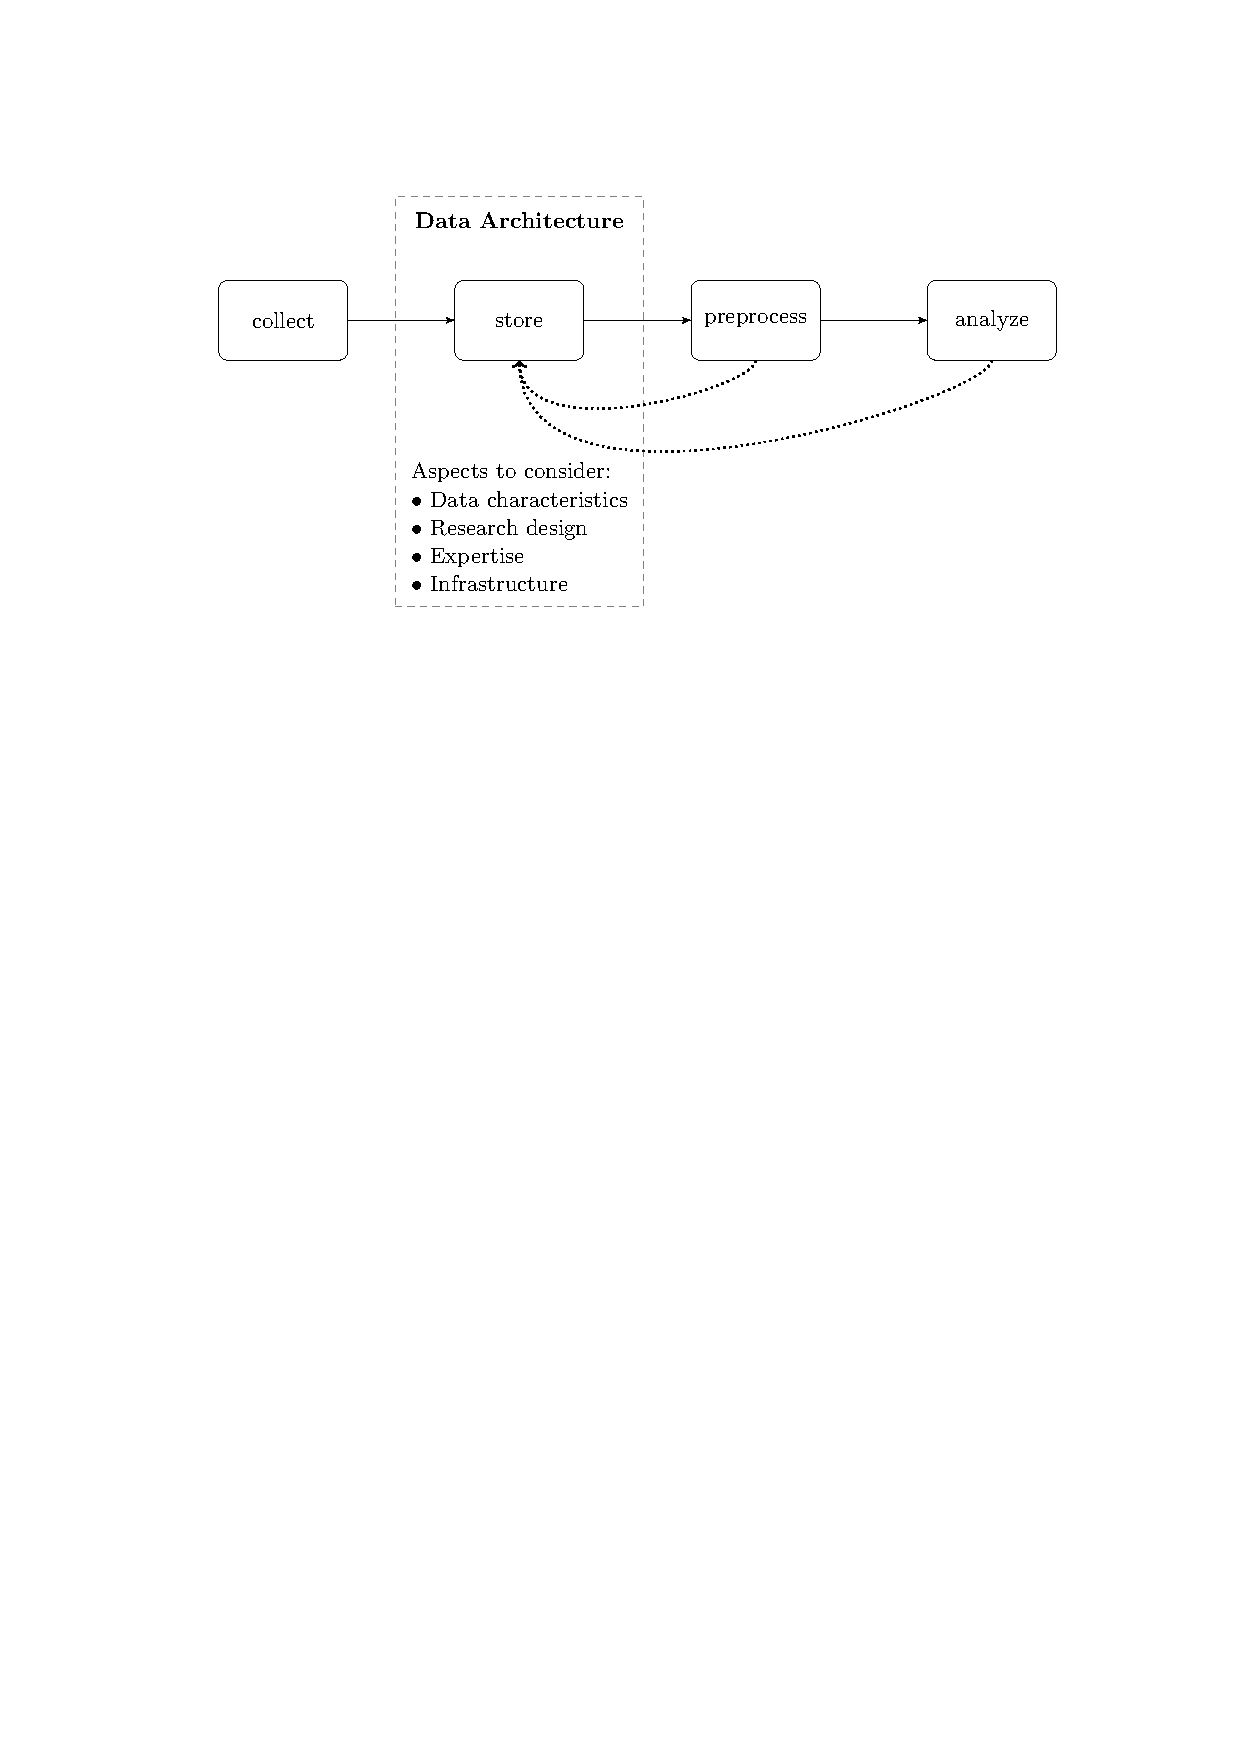
\includegraphics[width=\paperwidth,height=\paperheight,keepaspectratio]{guentheretal_fig1}}
\end{frame}




\begin{frame}{From retrieved data to enriched data}
	\makebox[\linewidth]{
		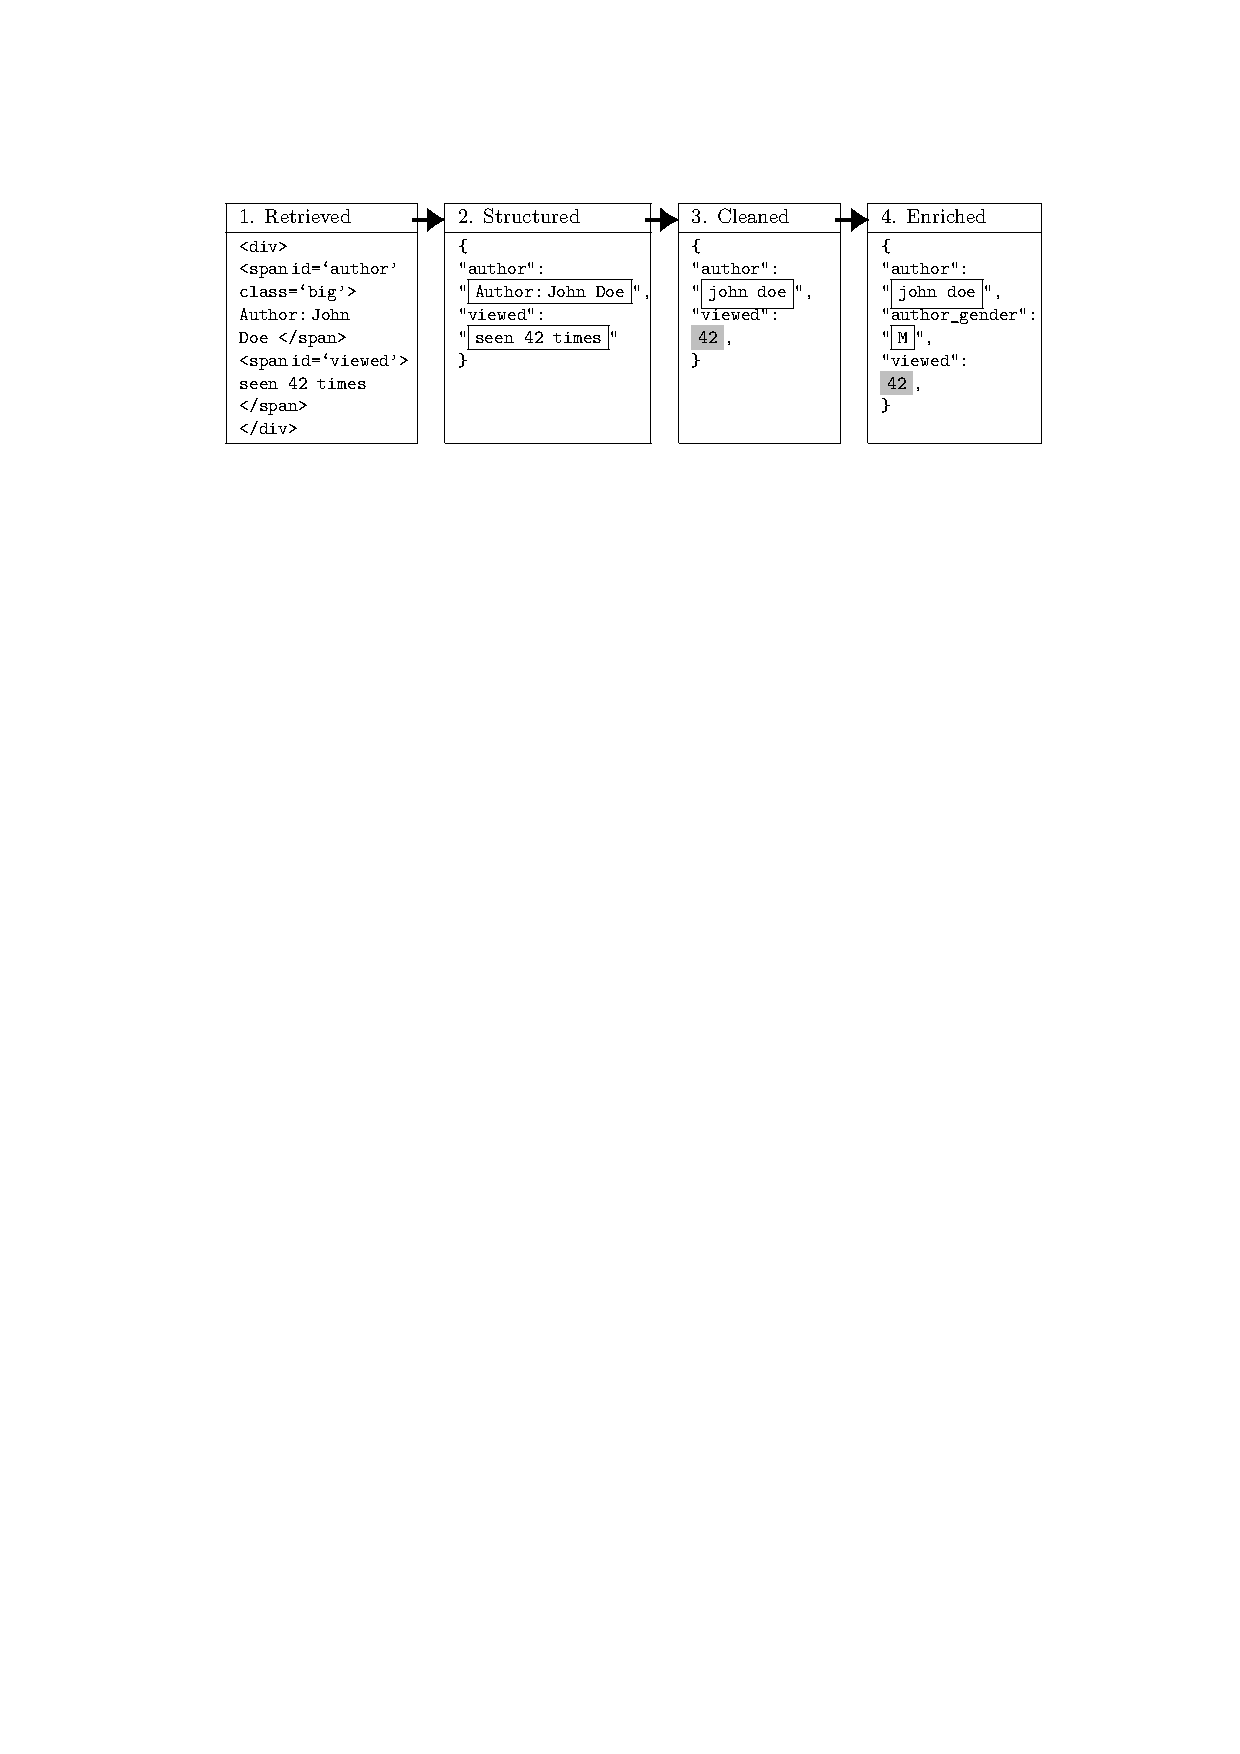
\includegraphics[width=\paperwidth,height=\paperheight,keepaspectratio]{guentheretal_fig3}}
\end{frame}

%
%
%
%\begin{frame}{Process and/or enrich}
%	\begin{block}{Word embeddings}
%	We did not really consider the \emph{meaning} of words
%		\begin{itemize}
%		\item Word embeddings can be trained on large corpora (e.g., whole wikipedia or a couple of years of newspaper coverage) 
%		\item The trained model allows you to calculate with words (hence, word vectors): $king-man+woman = ?$ 
%		\item You can find out whether documents are similar \emph{even if they do not use the same words} (Word Mover Distance)
%		\item $\Rightarrow$ word2vec (in gensim!), glove
%		\end{itemize}
%	\end{block}
%\end{frame}
%
%



\begin{frame}{Process and/or enrich}
	\begin{block}{Advanced NLP}
		We did a lot of BOW (and some part-of-speech (POS) tagging and named entity recognition (NER)), but we can do much more, such as 
		\begin{itemize}
			\item State-of-the-art Dependency Parsing to find out exact relationships
			$\Rightarrow$  spacy, stanza (stanford NLP)
                        \item \ldots
		\end{itemize}
	\end{block}
\end{frame}


 
\begin{frame}{Analyze/explain/predict}
	\begin{block}{More advanced modelling}
		We only did some basic statistical tests
		\begin{itemize}
			\item There are more advanced regression techniques and dimension-reduction techniques tailored to data that are, e.g., large-scale, sparse, have a lot of features, \ldots
			\item $\Rightarrow$ scikit-learn, statsmodels
		\end{itemize}
	\end{block}
\end{frame}


 
\begin{frame}{Analyze/explain/predict}
	\begin{block}{Really go into deep learning}
		We only got a brief intro to keras and to different archtectures -- there is a lot to learn here.
                \end{block}
\end{frame}






\subsection{Transformers}

\begin{frame}[standout]
If there is one thing that is really hot (as also mentioned in week 12 and by Luna today), then that's transformer models. Look into \texttt{huggingface} to get started!
\end{frame}

\begin{frame}{Some links}
\begin{itemize}
\item \url{https://nlp.seas.harvard.edu/2018/04/03/attention.html}
\item \url{http://jalammar.github.io/illustrated-transformer/}
\end{itemize}
\end{frame}


\section{Final project}

\begin{frame}[standout]
Talk to me about your plans!
\end{frame}

\begin{frame}{How will the grade be determined?}
Grading of the final project: 30\% for the report and the documentation of the notebook; 70\% for data, code, and analysis

\pause

\begin{block}{Report and documentation}
(see also syllabus)
\footnotesize
\begin{itemize}
\item Completeness and comprehensiveness
\item Quality of argumentation
\item Clear and correct presentation of and relevant selection of results
\item Correctness and appropriateness of conclusion and suggestions for future research
\item Outward appearance
\end{itemize}
\end{block}

\end{frame}



\begin{frame}{How will the grade be determined?}
Grading of the final project: 30\% for the report and the documentation of the notebook; 70\% for data, code, and analysis


\begin{block}{Data, code, and analysis}
(see also syllabus)
\footnotesize
\begin{itemize}
\item Covers techniques from most weeks
\item Coding style and efficiency
\item Follows best practices as you know \emph{at the end} of the course (i.e., if you learned a better technique later, you typically should use (also) the better technique)
\item Data quality and size (should be non-trivial; i.e., must make sense to use automated approach for it)
\item Correctness of analysis and decisions
\item Creativity, smart solutions and ideas, \ldots
\end{itemize}
\end{block}

\end{frame}

\begin{frame}[standout]
Being able to conduct all steps of your own computational social science research project is one of the main learning goals of this course. This gives you a lot of freedom, but also inevitably means that many of you will end up doing very different things -- and that reproducing some recipe is not what is tested and graded.
\end{frame}

\begin{frame}{Let's try to put some numbers on it}
Some hypothetical scenario's (as an \textbf{indication}):
\footnotesize

\begin{itemize}[<+>]
\item Existing dataset downloaded from Kaggle, limited NLP, simple basic LDA: $<5.0$
\item Existing dataset, but good and extensive NLP, extensive machine learning approaches; yet, not all best practices followed: $6-7$
\item Data aquired via APIs or webscraping, multiple NLP techniques applied, SML including extensive comparisons, hyperparameter tuning, visualizations of results, maybe some statistical tests for comparisons after enriching: $7-8$
\item Next to fulfilling all criteria, the projct solves a complex task that is going clearly beyond the specific examples used in class and/or in the take-home assignments (e.g., develops a complex web scraper for the data collection stage): $8+$
\end{itemize}
(all of this assuming that the methods are suitable to answer the RQ, otherwise the grade is of course lower)
\end{frame}


\begin{frame}[standout]
Rules of thumb: The more its mere replication, the lower the grade. The more you cover \emph{each} of the steps (today's slides) extensively, the higher the grade.

\end{frame}





\begin{frame}[standout]
Your questions?
\end{frame}





\begin{frame}[standout]
GOOD LUCK!
\end{frame}





\begin{frame}[allowframebreaks,plain]
\printbibliography
\end{frame}



\end{document}
